
\QCMautoevaluation{Pour chaque question, plusieurs réponses sont
  proposées.  Déterminer celles qui sont correctes.}

\begin{QCM}
  \begin{GroupeQCM}
    \begin{exercice}
      Si $T$ est le milieu d'un segment $[AD]$ et que $AD = 56$ mm alors \ldots
      \begin{ChoixQCM}{4}
      \item $T \in [AD]$
      
      et $TA = 28$ mm
      \item $TA = TD$
      \item \\[-1em]
      \includegraphics[width=2.6cm]{triangleATD}
      \item $[AD]$ est un diamètre du cercle de centre $T$ et de rayon 28 mm
      \end{ChoixQCM}
\begin{corrige}
     \reponseQCM{abd} 
   \end{corrige}
    \end{exercice}

  \begin{exercice}
      Si $ROSE$ est un losange alors \ldots
      \begin{ChoixQCM}{4}
      \item $[RE]$ est une diagonale
      \item $[OS]$ est une diagonale
      \item $[OS]$ est un côté
      \item $[RS]$ est une diagonale
      \end{ChoixQCM}
\begin{corrige}
     \reponseQCM{cd}
   \end{corrige}
    \end{exercice}

\begin{exercice}
      ABCD est une figure telle que (AB) est parlallèle à (CD), (AD) est parallèle à (BC), (AB) et (BC) sont perpendiculaires. ABCD est un:
      \begin{ChoixQCM}{4}
      \item carré
      \item losange
      \item rectangle
      \item parallélogramme
      \end{ChoixQCM}
\begin{corrige}
     \reponseQCM{c} 
   \end{corrige}
    \end{exercice}

\begin{exercice}
     Les côtés consécutifs d'un losange sont:
      \begin{ChoixQCM}{3}
      \item parallèles
      \item perpendiculaires
      \item de la même longueur
      \end{ChoixQCM}
\begin{corrige}
     \reponseQCM{c} 
   \end{corrige}
    \end{exercice}

\begin{exercice}
     Les diagonales d'un carré:
      \begin{ChoixQCM}{4}
      \item sont perpendiculaires
      \item sont parallèles
      \item ont la même longueur
      \item ont le même milieu
      \end{ChoixQCM}
\begin{corrige}
     \reponseQCM{acd} 
   \end{corrige}
    \end{exercice}

\begin{exercice}
      On sait que BLOC est un parallélogramme tel que (BO) et (LC) sont perpendiculaires. On peut dire que:
      \begin{ChoixQCM}{4}
      \item BLOC est un losange
      \item BLOC est un rectangle
      \item BLOC est un carré
      \item BLOC est un parallélogramme
      \end{ChoixQCM}
\begin{corrige}
     \reponseQCM{a} 
   \end{corrige}
    \end{exercice}

\begin{exercice}
      Un carré est un
      \begin{ChoixQCM}{4}
      \item losange
      \item rectangle
      \item parallélogramme
      \item quadrilatère
      \end{ChoixQCM}
\begin{corrige}
     \reponseQCM{abcd} 
   \end{corrige}
    \end{exercice}

\begin{exercice}
     On sait que ABCD est un parallélogramme tel que AC=BD. On peut en déduire que ABCD est un:
      \begin{ChoixQCM}{4}
      \item parallélogramme
      \item losange
      \item carré
      \item rectangle
      \end{ChoixQCM}
\begin{corrige}
     \reponseQCM{d} 
   \end{corrige}
    \end{exercice}

\begin{exercice}
À partir du codage du quadrilatère suivant, tracé à main levée : \hspace{0.5em} \raisebox{-0.5\height}{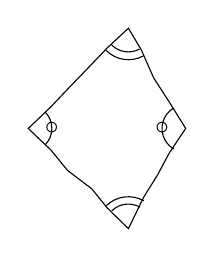
\begin{tikzpicture}[rotate=0,every node/.style={scale=1}]

\tikzstyle{MainLevee}=[decorate,decoration={random steps,amplitude=1pt,segment length=10pt}]

\coordinate (A) at (0,0);
\coordinate (B) at (45:1.8);
\coordinate (C) at (0:2);
\coordinate (D) at (-45:1.8);

\draw[MainLevee] (A) -- (B) -- (C) -- (D) --cycle;

\draw (45:0.3) arc (45:-45:0.3) node[midway]{$\circ$};
\draw (1.85,0.26) arc (119.74:240.27:0.3)node[midway]{$\circ$};

\draw (1.06,1.06) arc (-135:-61.74:0.3);
\draw (.99,.99) arc (-135:-61.74:0.4);
\draw (1.42,-1.0) arc (60.26:134:0.3);
\draw (1.47,-0.92) arc (60.26:134:0.4);

\end{tikzpicture}}, on peut affirmer que c'est un:
      \begin{ChoixQCM}{4}
      \item parallélogramme
      \item rectangle
      \item losange
      \item carré
      \end{ChoixQCM}
\begin{corrige}
     \reponseQCM{c} 
   \end{corrige}
    \end{exercice}
    
\end{GroupeQCM}
\end{QCM}

\begin{QCM}
  \begin{GroupeQCM}
\begin{exercice}
À partir du codage du quadrilatère suivant, tracé à main levée : \hspace{0.5em} \raisebox{-0.5\height}{\input{./Quadrilateres/figures/QCM_MainLevee_2}}, on peut affirmer que c'est un:
      \begin{ChoixQCM}{4}
      \item parallélogramme
      \item rectangle
      \item losange
      \item carré
      \end{ChoixQCM}
\begin{corrige}
     \reponseQCM{c} 
   \end{corrige}
    \end{exercice}

\begin{exercice}
À partir du codage du quadrilatère suivant, tracé à main levée : \hspace{0.5em} \raisebox{-0.5\height}{\input{./Quadrilateres/figures/QCM_MainLevee_3}}, on peut affirmer que c'est un:
      \begin{ChoixQCM}{4}
      \item parallélogramme
      \item rectangle
      \item losange
      \item carré
      \end{ChoixQCM}
\begin{corrige}
     \reponseQCM{c} 
   \end{corrige}
    \end{exercice}

\begin{exercice}
À partir du codage du quadrilatère suivant, tracé à main levée : \hspace{0.5em} \raisebox{-0.5\height}{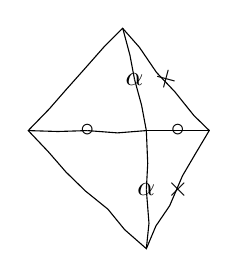
\begin{tikzpicture}[rotate=0,every node/.style={scale=1}]

\tikzstyle{MainLevee}=[decorate,decoration={random steps,amplitude=1pt,segment length=10pt}]

\coordinate (A) at (0,0);
\coordinate (B) at (1.2,1.3);
\coordinate (C) at (2.3,0);
\coordinate (D) at (1.5,-1.5);
\coordinate (O) at (1.5,0); %le centre du losange

%%%%%Les marques d'égalité de longueurs sur les diagonales :
\coordinate (A') at (0.75,0); %le milieu de la diagonale [AO]
\coordinate (B') at (1.35,0.65);
\coordinate (C') at (1.9,0);
\coordinate (D') at (1.5,-0.75);
\node at (A'){$\circ$};
\node at (B'){$\alpha$};
\node at (C'){$\circ$};
\node at (D'){$\alpha$};
%%% Les marques d'égalité de longueurs sur 2 côtés
\draw (1.75,0.65) node[rotate=30] {$\times$};
\draw (1.9,-0.75) node[rotate=0] {$\times$};

\draw[MainLevee] (A) -- (B) -- (C) -- (D) --cycle;

\draw[MainLevee] (A)--(A'); 
\draw[MainLevee] (A')--(O);
\draw[MainLevee] (B)--(B'); 
\draw[MainLevee] (B')--(O);
\draw[MainLevee] (C)--(C'); 
\draw[MainLevee] (C')--(O);
\draw[MainLevee] (D)--(D'); 
\draw[MainLevee] (D')--(O);

\end{tikzpicture}}, on peut affirmer que c'est un:
      \begin{ChoixQCM}{4}
      \item parallélogramme
      \item rectangle
      \item losange
      \item carré
      \end{ChoixQCM}
\begin{corrige}
     \reponseQCM{c} 
   \end{corrige}
    \end{exercice}

\end{GroupeQCM}
\end{QCM}

  
